\documentclass[aspectratio=169, t, 8pt]{beamer}

%------configurando acentos-----------
\usepackage[utf8]{inputenc}
\usepackage[brazil]{babel}

\usepackage{graphicx}

%-------Estilos Beamer---------------
\usetheme{metropolis}
%\usecolortheme{crane}
%coment
%\usefonttheme{serif}
\linespread{1.2}

% Personalização de Cores (Exemplo: Minimal Teal)
% Cores Base
\definecolor{BgCanvas}{HTML}{F9F9FB}      % Off-white muito suave
\definecolor{MainText}{HTML}{2B2D42}      % Grafite escuro para alta legibilidade
\definecolor{PrimaryAccent}{HTML}{4A6FA5} % Az
\definecolor{SunCoastFg}{HTML}{F2A154}
% --- CONFIGURAÇÕES DE TEMA BEAMER ---
%\usetheme{metropolis}

\setbeamertemplate{itemize item}{\textcolor{MainText}{$\bullet$}}
\setbeamertemplate{itemize subitem}{\textcolor{MainText}{\scriptsize$\circ$}}
\setbeamertemplate{itemize 3rditem}{\textcolor{MainText}{\tiny$\blacksquare$}}

\setbeamercolor{background canvas}{bg=BgCanvas}
\setbeamercolor{normal text}{fg=MainText}
\setbeamercolor{frametitle}{bg=SunCoastFg, fg=BgCanvas}
\setbeamercolor{title}{fg=MainText}
\setbeamercolor{subtitle}{fg=PrimaryAccent}
\setbeamercolor{structure}{fg=PrimaryAccent}

% Remove a linha amarela padrão do Metropolis sob o título
\setbeamertemplate{title separator}{}
\setbeamertemplate{progress bar in section page}{}


%--------Dados do Documento
\title{Matemática: Lista de Exercícios}
\author{prof. Eduardo}
\institute{Pré-Universitário Oficina do Saber / UFF}
\date{\today}


%-------- Pacotes Matemática -------------
\usepackage{amsmath}
\usepackage{amsthm}
\usepackage{amsfonts}
\usepackage{amssymb}
\usepackage{xfrac}
\usepackage{thmtools}

%-------- Configuração Listas---------
% \usepackage{enumitem}
\usepackage[inline]{enumitem}

\setcounter{tocdepth}{2}

\newcounter{questaovest}
\newcommand{\vest}[1]{\stepcounter{questaovest}\item[\textbf{Questão \arabic{questaovest}} (#1):]}
\setlist[enumerate]{
    align=left,
    leftmargin=1.8em,
    itemindent=1.8em
    }

\setlist[enumerate,2]{
    label=\alph*.,
    font=\bfseries,
    itemsep=0.1pt,
    labelsep=0em,
    parsep=0pt,
    leftmargin=0em,
    }

%------------- Atalho para imagens ------------
\graphicspath{{../../src/img/semana09/}}


\begin{document}

\begin{frame} %capa
        \vspace*{\fill}
            
            \begin{columns}[c]
                \begin{column}{0.5\textwidth}
                    {\usebeamerfont{title}\usebeamercolor[fg]{title}\inserttitle}\vspace{0.2cm}
                    
                    {\usebeamerfont{subtitle}\usebeamercolor[fg]{subtitle}\insertsubtitle}\vspace{0.5cm}

                {\usebeamerfont{author}\insertauthor}\vspace{0.3cm}

                {\usebeamerfont{institute}\insertinstitute}\vspace{0.3cm}

                {\usebeamerfont{date}\insertdate}
            \end{column}
            
            
            \begin{column}{0.4\textwidth}
                \centering
                
\includegraphics[width=0.4\textwidth]{../logo_ofSaber.png}

                \vspace{.4cm}
                \vspace*{\fill}
        \begin{columns}[c]
            \begin{column}{.5\textwidth}
                \centering
\includegraphics[width=.5\textwidth]{../Proex02c.png}
            \end{column}
            \begin{column}{.5\textwidth}
                \centering
\includegraphics[width=0.4\textwidth]{../Logo_UFF.png}
            \end{column}
        \end{columns}
        \vspace*{\fill}
            \end{column}
        \end{columns}
    \vspace*{\fill}
    \end{frame}
    
        % {
        %     \usebackgroundtemplate{
        %     \includegraphics[width=\paperwidth]{slide_02_contracapa.png}}
        %     \begin{frame}[plain]                
        %     \end{frame}
        % }


    \begin{frame} %Questão 01-D
        \frametitle{Geometria Espacial: Volume}
        \vspace{-1.2em}
        \begin{enumerate}
            \begin{columns}
                \begin{column}{.9\textwidth}
                    \vest{UFRGS-2010} Um reservatório tem forma de um cilindro circular reto com duas semiesferas acopladas em suas extremidades, conforme representado na figura a seguir.

                    \begin{columns}[totalwidth=\textwidth,T]
                        \begin{column}{.3\textwidth}
                            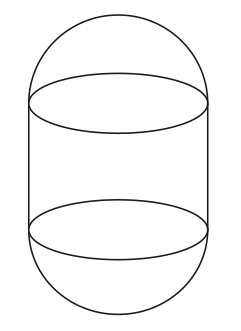
\includegraphics[width=.9\textwidth]{monitoria_q1.png}
                        \end{column}

                        \begin{column}{.65\textwidth}
                            O diâmetro da base e a altura do cilindro medem, cada um, $4$ dm, e o volume de uma esfera de raio $r$ é $\frac{4}{3}\pi r^{3}$.

                            Dentre as opções a seguir, o valor mais próximo da capacidade do reservatório, em litros, é

                            \vspace{1em}

                            \raggedleft
                            \begin{minipage}{\textwidth}
                                \begin{enumerate*}[itemjoin={\hfill}]
                                    \item 50.
                                    \item 60.
                                    \item 70.
                                    \item 80.
                                    \item 90.
                                \end{enumerate*}
                            \end{minipage}
                        \end{column}
                    \end{columns}
                \end{column}
            \end{columns}
        \end{enumerate}
    \end{frame}

    \begin{frame}{Contagem} %E
        \begin{columns}[totalwidth=.9\textwidth]
            \begin{column}{\textwidth}
                \begin{enumerate}
                    \vest{IFAL-2018} Em uma civilização antiga, o alfabeto tinha apenas três letras. Na linguagem dessa civilização, as palavras tinham de uma a quatro letras. Quantas palavras poderiam existir na linguagem dessa civilização?

                    \begin{enumerate}
                        \item 4
                        \item 12
                        \item 16
                        \item 40
                        \item 120
                    \end{enumerate}
                \end{enumerate}
            \end{column}
        \end{columns}
    \end{frame}

    \begin{frame}{Geometria Espacial: Volume} %D
        \begin{columns}[totalwidth=.9\textwidth]
            \begin{column}{\textwidth}
                \begin{enumerate}
                    \vest{UNEM-2016} Em regiões agrícolas, é comum a presença de silos para armazenamento e secagem da produção de grãos, no formato de um cilindro reto, sobreposta por um cone, e dimensões indicadas na figura. O silo fica cheio e o transporte dos grãos é feito em caminhões de carga cuja capacidade é de $20 \text{ m}^3$. Uma região possui um silo cheio e apenas um caminhão para transportar os grãos para a usina de beneficiamento.

                    \begin{columns}[totalwidth=\textwidth, T]
                        \begin{column}{.4\textwidth}
                            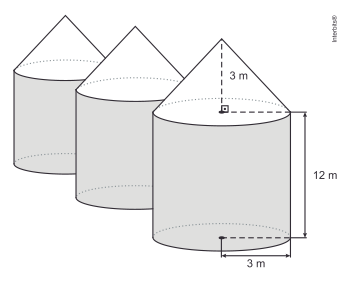
\includegraphics[width=\textwidth]{monitoria_03.png}
                        \end{column}
                        \begin{column}{.5\textwidth}
                            Utilize 3 como aproximação para $\pi$.
                            
                            O número mínimo de viagens que o caminhão precisará fazer para transportar todo o volume de grãos armazenados no silo é
                            
                            \vspace{1.2em}

                            \raggedright

                            \begin{minipage}{.8\textwidth}
                                \begin{enumerate*}[itemjoin={\hfill}]
                                    \item 6.
                                    \item 16.
                                    \item 17.
                                    \item 18.
                                    \item 21.
                                \end{enumerate*}
                            \end{minipage}
                        \end{column}
                    \end{columns}
                \end{enumerate}
            \end{column}
        \end{columns}
    \end{frame}

    \begin{frame}{Princípio de Arquimedes}
      \begin{columns}[totalwidth=.9\textwidth]
        \begin{column}{\textwidth}
            \begin{enumerate}
                \vest{UFU-2018} Um recipiente, no formato de um cilindro circular reto de raio de base $r\text{ cm}$, possui um líquido solvente em seu interior. A altura $h$ desse solvente presente no recipiente é igual a $\frac{16}{3}\text{ cm}$, conforme ilustra a {\it Figura 1}.

                Quando uma peça maciça, no formato de uma esfera de raio igual a $3 \text{ cm}$, é mergulhada nesse recipiente até encostar no fundo, observa-se que o solvente cobre exatamente a esfera, conforme ilustra a {\it Figura 2}.

                \vspace{1.2em}

                \begin{columns}[totalwidth=\textwidth,T]
                    \begin{column}{.45\textwidth}
                        \centering
                        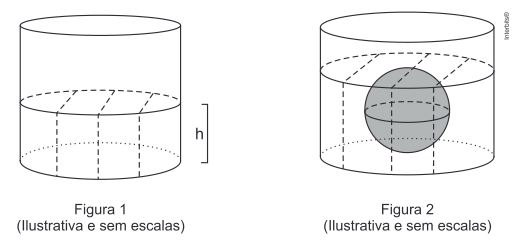
\includegraphics[width=\textwidth]{monitoria_q4.png}
                    \end{column}
                    \begin{column}{.45\textwidth}
                        Segundo as condições apresentadas, o raio r, em cm, é igual a:
                        
                        \vspace{1em}

                        \raggedright
                        \begin{minipage}{.8\textwidth}
                            \begin{enumerate*}[itemjoin={\hfill}]
                                \item $4 \sqrt{3}$
                                \item $2 \sqrt{7}$
                                \item $5 \sqrt{2}$
                                \item $3 \sqrt{6}$
                            \end{enumerate*}
                        \end{minipage}
                    \end{column}
                \end{columns}
            \end{enumerate}
        \end{column}
      \end{columns}  
    \end{frame}

    \begin{frame}{Semelhança de Triângulos}
        \begin{columns}[totalwidth=.9\textwidth]
            \begin{column}{\textwidth}
                \begin{enumerate}
                    \vest{FATEC-1999} Na figura a seguir, o triângulo ABC é retângulo e isósceles e o retângulo nele inscrito tem lados que medem $4$ cm e $2$ cm.

                    \vspace{1.2em}

                    \begin{columns}[totalwidth=\textwidth, T]
                        \begin{column}{.25\textwidth}
                            \centering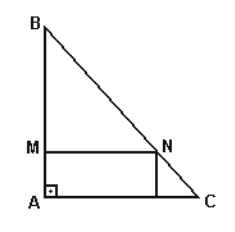
\includegraphics[width=\textwidth]{monitoria_q05.png}
                        \end{column}
                        \begin{column}{.7\textwidth}
                            O perímetro do triângulo $MNB$ é

                            \vspace{1em}

                            \raggedright
                            \begin{minipage}{\textwidth}
                                \begin{enumerate*}[itemjoin={\hfill}]
                                    \item $8 \text{ cm}$
                                    \item $12 \text{ cm}$
                                    \item $\left( 8 + \sqrt{2}\right) \text{ cm}$
                                    \item $4 \left( 2 + \sqrt{2}\right) \text{ cm}$
                                \end{enumerate*}
                            \end{minipage}
                        \end{column}
                    \end{columns}
                \end{enumerate}
            \end{column}
        \end{columns}
    \end{frame}
\end{document}